\section{レーザー測定の方法と使用装置}
\subsection{レーザーの性能}
今回のLGAD検出器の増幅率の測定においては、図\ref{fg:Laser} の赤外線パルスレーザーを使用する。
このレーザーは、NKT Photonics社のKATANA 10 \cite{KATANA10}で、レーザーの性能について 表\ref{tab:Laser_performance} にまとめた。

\begin{figure}[h]
    \begin{minipage}[c]{0.45\linewidth}
        \centering
        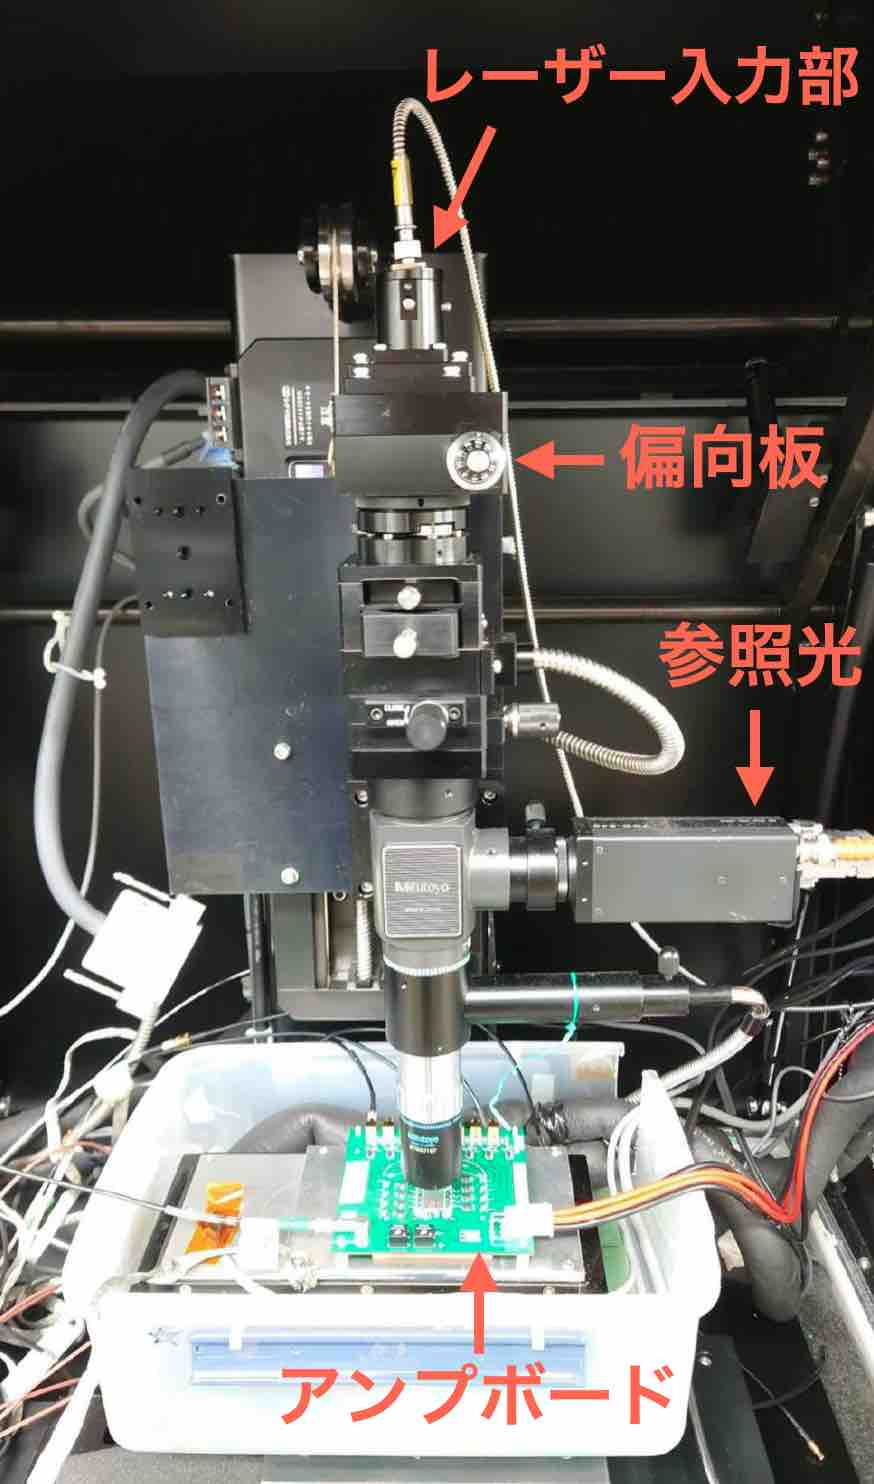
\includegraphics[width=5cm]{fig/ch3/Laser.jpg}
        \caption{赤外線パルスレーザー本体}
        \label{fg:Laser}
    \end{minipage}
    \begin{minipage}[c]{0.45\linewidth}   %*** 表の書き方
        \def\@captype{table}
        \tblcaption{赤外線パルスレーザーの性能表}
        \centering
        \begin{tabular}{cc}
            \hline
            モデル & KATANA 10  \\ \hline \hline
            波長 & $1064 \pm 2\:\rm{nm}$  \\ 
            パルス幅 & $35 \pm 15\:\rm{ps}$  \\ 
            平均出力 & $>10\:\rm{mW}\;\rm{at}\;1\:\rm{MHz}$  \\ 
            繰り返し周波数 & $20\:-\:80\:\rm{MHz}$  \\ 
            スペクトルバンド幅 FWHM & $<0.4\:\rm{nm}$  \\ 
            振幅ノイズ & $<4\:\%\;\rm{rms}$  (10時間)\\ 
            タイミングジッタ & $<10\:\rm{ps}$  \\ \hline
        \end{tabular}
        \label{tab:Laser_performance}
    \end{minipage}
\end{figure}

